\documentclass[sigplan,review,anonymous]{acmart}
\settopmatter{printfolios=true,printccs=false,printacmref=false}
\setcopyright{none}
\acmConference[LCTES '27]{ACM SIGPLAN/SIGBED International Conference on Languages, Compilers, and Tools for Embedded Systems}{2027}{}

\usepackage{booktabs}
\usepackage{xspace}
% Generated by paper/make_numbers.py from outputs/v3_1 and data/v3_1. Do not edit.
\newcommand{\CurveGAOne}{1.537}
\newcommand{\CurveGATen}{1.079}
\newcommand{\CurveGATwoHundred}{0.969}
\newcommand{\CurveOracleOne}{1.142}
\newcommand{\CurveOracleTen}{1.136}
\newcommand{\CurveOracleTwoHundred}{1.096}
\newcommand{\CurvePanOne}{1.282}
\newcommand{\CurvePanTen}{1.114}
\newcommand{\CurvePanTwoHundred}{0.966}
\newcommand{\CurvePredOnceOne}{1.169}
\newcommand{\CurvePredOnceTen}{1.165}
\newcommand{\CurvePredOnceTwoHundred}{1.133}
\newcommand{\CurveRepredictOne}{1.203}
\newcommand{\CurveRepredictTen}{1.194}
\newcommand{\CurveRepredictTwoHundred}{1.173}
\newcommand{\CurveStaticOne}{1.200}
\newcommand{\CurveStaticTen}{1.197}
\newcommand{\CurveStaticTwoHundred}{1.151}
\newcommand{\HFourHi}{1.170}
\newcommand{\HFourLo}{1.053}
\newcommand{\HFourLosses}{88}
\newcommand{\HFourOther}{ga}
\newcommand{\HFourP}{1.00}
\newcommand{\HFourPHolm}{1.00}
\newcommand{\HFourPct}{-10.7}
\newcommand{\HFourPrograms}{129}
\newcommand{\HFourRatio}{1.107}
\newcommand{\HFourTies}{3}
\newcommand{\HFourWins}{38}
\newcommand{\HFourWorse}{10.7}
\newcommand{\HOneHi}{0.976}
\newcommand{\HOneLo}{0.919}
\newcommand{\HOneLosses}{26}
\newcommand{\HOneP}{1.3\times 10^{-9}}
\newcommand{\HOnePHolm}{2.6\times 10^{-9}}
\newcommand{\HOnePct}{5.1}
\newcommand{\HOnePrograms}{129}
\newcommand{\HOneRatio}{0.949}
\newcommand{\HOneTies}{8}
\newcommand{\HOneWins}{95}
\newcommand{\HOneWorse}{-5.1}
\newcommand{\HThreeBetter}{127}
\newcommand{\HThreeGap}{39}
\newcommand{\HThreeMaeModel}{0.0051}
\newcommand{\HThreeMaeStatic}{0.0084}
\newcommand{\HThreeP}{1.0\times 10^{-21}}
\newcommand{\HThreePHolm}{4.1\times 10^{-21}}
\newcommand{\HThreePrograms}{129}
\newcommand{\HThreeRsq}{0.50}
\newcommand{\HThreeWorse}{2}
\newcommand{\HTwoHi}{0.34}
\newcommand{\HTwoLo}{0.27}
\newcommand{\HTwoP}{2.7\times 10^{-21}}
\newcommand{\HTwoPHolm}{8.0\times 10^{-21}}
\newcommand{\HTwoPrograms}{123}
\newcommand{\HTwoRho}{0.29}
\newcommand{\LLVMVersion}{21.1.8}
\newcommand{\LevelOOne}{1.113}
\newcommand{\LevelOThree}{1.300}
\newcommand{\LevelOTwo}{1.253}
\newcommand{\LevelOZero}{2.661}
\newcommand{\LevelOs}{1.028}
\newcommand{\LevelOz}{1.000}
\newcommand{\MDynHi}{1.006}
\newcommand{\MDynLo}{0.783}
\newcommand{\MDynLosses}{52}
\newcommand{\MDynP}{0.13}
\newcommand{\MDynPct}{7.9}
\newcommand{\MDynPrograms}{129}
\newcommand{\MDynRatio}{0.921}
\newcommand{\MDynTies}{17}
\newcommand{\MDynWins}{60}
\newcommand{\MDynWorse}{-7.9}
\newcommand{\MGAOThreeDynHi}{1.265}
\newcommand{\MGAOThreeDynLo}{1.135}
\newcommand{\MGAOThreeDynLosses}{119}
\newcommand{\MGAOThreeDynP}{1.00}
\newcommand{\MGAOThreeDynPct}{-19.4}
\newcommand{\MGAOThreeDynPrograms}{129}
\newcommand{\MGAOThreeDynRatio}{1.194}
\newcommand{\MGAOThreeDynTies}{0}
\newcommand{\MGAOThreeDynWins}{10}
\newcommand{\MGAOThreeDynWorse}{19.4}
\newcommand{\MGAOThreeRuntimeHi}{1.315}
\newcommand{\MGAOThreeRuntimeLo}{1.116}
\newcommand{\MGAOThreeRuntimeLosses}{68}
\newcommand{\MGAOThreeRuntimeP}{1.00}
\newcommand{\MGAOThreeRuntimePct}{-20.5}
\newcommand{\MGAOThreeRuntimePrograms}{89}
\newcommand{\MGAOThreeRuntimeRatio}{1.205}
\newcommand{\MGAOThreeRuntimeTies}{0}
\newcommand{\MGAOThreeRuntimeWins}{21}
\newcommand{\MGAOThreeRuntimeWorse}{20.5}
\newcommand{\MGAOThreeSizeHi}{0.825}
\newcommand{\MGAOThreeSizeLo}{0.728}
\newcommand{\MGAOThreeSizeLosses}{27}
\newcommand{\MGAOThreeSizeP}{6.1\times 10^{-13}}
\newcommand{\MGAOThreeSizePct}{22.4}
\newcommand{\MGAOThreeSizePrograms}{129}
\newcommand{\MGAOThreeSizeRatio}{0.776}
\newcommand{\MGAOThreeSizeTies}{6}
\newcommand{\MGAOThreeSizeWins}{96}
\newcommand{\MGAOThreeSizeWorse}{-22.4}
\newcommand{\MGAOzIRHi}{0.987}
\newcommand{\MGAOzIRLo}{0.950}
\newcommand{\MGAOzIRLosses}{30}
\newcommand{\MGAOzIRP}{3.3\times 10^{-9}}
\newcommand{\MGAOzIRPct}{3.1}
\newcommand{\MGAOzIRPrograms}{129}
\newcommand{\MGAOzIRRatio}{0.969}
\newcommand{\MGAOzIRTies}{7}
\newcommand{\MGAOzIRWins}{92}
\newcommand{\MGAOzIRWorse}{-3.1}
\newcommand{\MGAOzSizeHi}{1.202}
\newcommand{\MGAOzSizeLo}{1.139}
\newcommand{\MGAOzSizeLosses}{119}
\newcommand{\MGAOzSizeP}{1.00}
\newcommand{\MGAOzSizePct}{-16.6}
\newcommand{\MGAOzSizePrograms}{129}
\newcommand{\MGAOzSizeRatio}{1.166}
\newcommand{\MGAOzSizeTies}{6}
\newcommand{\MGAOzSizeWins}{4}
\newcommand{\MGAOzSizeWorse}{16.6}
\newcommand{\MRuntimeHi}{1.004}
\newcommand{\MRuntimeLo}{0.812}
\newcommand{\MRuntimeLosses}{38}
\newcommand{\MRuntimeP}{0.03}
\newcommand{\MRuntimePct}{7.9}
\newcommand{\MRuntimePrograms}{89}
\newcommand{\MRuntimeRatio}{0.921}
\newcommand{\MRuntimeTies}{0}
\newcommand{\MRuntimeWins}{51}
\newcommand{\MRuntimeWorse}{-7.9}
\newcommand{\MSizeAHi}{0.956}
\newcommand{\MSizeALo}{0.901}
\newcommand{\MSizeALosses}{29}
\newcommand{\MSizeAP}{1.5\times 10^{-7}}
\newcommand{\MSizeAPct}{7.0}
\newcommand{\MSizeAPrograms}{129}
\newcommand{\MSizeARatio}{0.930}
\newcommand{\MSizeATies}{24}
\newcommand{\MSizeATwoHundredHi}{0.936}
\newcommand{\MSizeATwoHundredLo}{0.884}
\newcommand{\MSizeATwoHundredLosses}{14}
\newcommand{\MSizeATwoHundredP}{2.5\times 10^{-12}}
\newcommand{\MSizeATwoHundredPct}{9.0}
\newcommand{\MSizeATwoHundredPrograms}{129}
\newcommand{\MSizeATwoHundredRatio}{0.910}
\newcommand{\MSizeATwoHundredTies}{47}
\newcommand{\MSizeATwoHundredWins}{68}
\newcommand{\MSizeATwoHundredWorse}{-9.0}
\newcommand{\MSizeAWins}{76}
\newcommand{\MSizeAWorse}{-7.0}
\newcommand{\MSizeXHi}{0.977}
\newcommand{\MSizeXLo}{0.921}
\newcommand{\MSizeXLosses}{31}
\newcommand{\MSizeXP}{4.1\times 10^{-6}}
\newcommand{\MSizeXPct}{5.0}
\newcommand{\MSizeXPrograms}{129}
\newcommand{\MSizeXRatio}{0.950}
\newcommand{\MSizeXTies}{22}
\newcommand{\MSizeXWins}{76}
\newcommand{\MSizeXWorse}{-5.0}
\newcommand{\NCBench}{12}
\newcommand{\NCandidates}{156}
\newcommand{\NExpFailed}{0}
\newcommand{\NExperiments}{312{,}825}
\newcommand{\NInteractionRows}{2{,}741{,}508}
\newcommand{\NMeasured}{18{,}645}
\newcommand{\NOwn}{24}
\newcommand{\NPairs}{462}
\newcommand{\NPasses}{22}
\newcommand{\NPolyBench}{30}
\newcommand{\NPrograms}{129}
\newcommand{\NReps}{4}
\newcommand{\NRuntimeBinaries}{6{,}432}
\newcommand{\NRuntimeReliable}{89}
\newcommand{\NSnapshots}{5}
\newcommand{\NTestSuite}{63}
\newcommand{\OutputFailures}{0}
\newcommand{\PassList}{\texttt{adce}, \texttt{correlated-propagation}, \texttt{dce}, \texttt{dse}, \texttt{early-cse}, \texttt{gvn}, \texttt{indvars}, \texttt{inline}, \texttt{instcombine}, \texttt{jump-threading}, \texttt{licm}, \texttt{loop-deletion}, \texttt{loop-rotate}, \texttt{loop-unroll}, \texttt{loop-vectorize}, \texttt{mem2reg}, \texttt{memcpyopt}, \texttt{reassociate}, \texttt{sccp}, \texttt{simplifycfg}, \texttt{slp-vectorizer}, \texttt{sroa}}
\newcommand{\PlateauGA}{31.1}
\newcommand{\PlateauOpenTuner}{35.2}
\newcommand{\PlateauOracle}{1.1}
\newcommand{\PlateauPan}{14.1}
\newcommand{\PlateauPredOnce}{0.4}
\newcommand{\PlateauRepredict}{0.0}
\newcommand{\PlateauStatic}{2.6}
\newcommand{\PreregSha}{71e6f03d91828c91d7fa1952af322cd1fb505c748735c92e580d1b5d97dff40e}
\newcommand{\PreregShaShort}{71e6f03d91828c91}
\newcommand{\RankModelSTwo}{0.77}
\newcommand{\RankModelSZero}{0.90}
\newcommand{\RankStaticSTwo}{0.71}
\newcommand{\RankStaticSZero}{0.83}
\newcommand{\RhoOneFour}{0.56}
\newcommand{\RhoOneThree}{0.58}
\newcommand{\RhoOneTwo}{0.58}
\newcommand{\RhoThreeFour}{0.78}
\newcommand{\RhoTwoFour}{0.78}
\newcommand{\RhoTwoThree}{1.00}
\newcommand{\RhoZeroFour}{0.32}
\newcommand{\RhoZeroOne}{0.32}
\newcommand{\RhoZeroThree}{0.29}
\newcommand{\RhoZeroTwo}{0.29}
\newcommand{\RuntimeCV}{1.9}
\newcommand{\RuntimeNoisy}{805}
\newcommand{\RuntimeNoisyPct}{13}
\newcommand{\SgeClassErrSZero}{8}
\newcommand{\SgeRhoSZero}{0.61}
\newcommand{\SgeTopkSZero}{60}
\newcommand{\SparseFour}{88}
\newcommand{\SparseOne}{87}
\newcommand{\SparseThree}{88}
\newcommand{\SparseTwo}{88}
\newcommand{\SparseZero}{81}
\newcommand{\Threshold}{0.005}
\newcommand{\VdPair}{19}
\newcommand{\VdPairCtx}{24}
\newcommand{\VdProg}{56}
\newcommand{\VdProgHi}{60}
\newcommand{\VdProgLo}{49}
\newcommand{\XOnceEFiveHi}{1.057}
\newcommand{\XOnceEFiveLo}{0.953}
\newcommand{\XOnceEFiveLosses}{76}
\newcommand{\XOnceEFiveP}{0.77}
\newcommand{\XOnceEFivePct}{-0.3}
\newcommand{\XOnceEFivePrograms}{129}
\newcommand{\XOnceEFiveRatio}{1.003}
\newcommand{\XOnceEFiveTies}{5}
\newcommand{\XOnceEFiveWins}{48}
\newcommand{\XOnceEFiveWorse}{0.3}
\newcommand{\XOnceEOneHi}{0.943}
\newcommand{\XOnceEOneLo}{0.879}
\newcommand{\XOnceEOneLosses}{39}
\newcommand{\XOnceEOneP}{3.6\times 10^{-8}}
\newcommand{\XOnceEOnePct}{8.9}
\newcommand{\XOnceEOnePrograms}{129}
\newcommand{\XOnceEOneRatio}{0.911}
\newcommand{\XOnceEOneTies}{1}
\newcommand{\XOnceEOneWins}{89}
\newcommand{\XOnceEOneWorse}{-8.9}
\newcommand{\XOracleEOneHi}{0.922}
\newcommand{\XOracleEOneLo}{0.859}
\newcommand{\XOracleEOneLosses}{32}
\newcommand{\XOracleEOneP}{3.5\times 10^{-10}}
\newcommand{\XOracleEOnePct}{10.9}
\newcommand{\XOracleEOnePrograms}{129}
\newcommand{\XOracleEOneRatio}{0.891}
\newcommand{\XOracleEOneTies}{1}
\newcommand{\XOracleEOneWins}{96}
\newcommand{\XOracleEOneWorse}{-10.9}
\newcommand{\XOracleGAHi}{1.116}
\newcommand{\XOracleGALo}{1.001}
\newcommand{\XOracleGALosses}{57}
\newcommand{\XOracleGAP}{0.26}
\newcommand{\XOracleGAPct}{-5.2}
\newcommand{\XOracleGAPrograms}{129}
\newcommand{\XOracleGARatio}{1.052}
\newcommand{\XOracleGATies}{3}
\newcommand{\XOracleGAWins}{69}
\newcommand{\XOracleGAWorse}{5.2}
\newcommand{\XRepEOneHi}{0.972}
\newcommand{\XRepEOneLo}{0.904}
\newcommand{\XRepEOneLosses}{60}
\newcommand{\XRepEOneP}{0.01}
\newcommand{\XRepEOnePct}{6.2}
\newcommand{\XRepEOnePrograms}{129}
\newcommand{\XRepEOneRatio}{0.938}
\newcommand{\XRepEOneTies}{1}
\newcommand{\XRepEOneWins}{68}
\newcommand{\XRepEOneWorse}{-6.2}
\newcommand{\XRepOnceHi}{1.044}
\newcommand{\XRepOnceLo}{1.007}
\newcommand{\XRepOnceLosses}{79}
\newcommand{\XRepOnceP}{1.00}
\newcommand{\XRepOncePct}{-2.5}
\newcommand{\XRepOncePrograms}{129}
\newcommand{\XRepOnceRatio}{1.025}
\newcommand{\XRepOnceTies}{14}
\newcommand{\XRepOnceWins}{36}
\newcommand{\XRepOnceWorse}{2.5}
\newcommand{\XRepStaticHi}{1.014}
\newcommand{\XRepStaticLo}{0.983}
\newcommand{\XRepStaticLosses}{63}
\newcommand{\XRepStaticP}{0.35}
\newcommand{\XRepStaticPct}{0.2}
\newcommand{\XRepStaticPrograms}{129}
\newcommand{\XRepStaticRatio}{0.998}
\newcommand{\XRepStaticTies}{13}
\newcommand{\XRepStaticWins}{53}
\newcommand{\XRepStaticWorse}{-0.2}

\newcommand{\Oz}{\texttt{-Oz}\xspace}
\newcommand{\Othree}{\texttt{-O3}\xspace}
\newcommand{\Otwo}{\texttt{-O2}\xspace}
\newcommand{\E}{\ensuremath{E}\xspace}

\begin{document}

\title{One Graph Does Not Fit All: Program-Specific and Drifting Pass Interactions in LLVM}

\author{Anonymous Author(s)}
\affiliation{\institution{Anonymous Institution}\country{}}

\begin{abstract}
Recent phase-ordering methods summarise pairwise pass interactions in a single graph learned from
a training corpus and apply it to every program. We test that assumption in LLVM with a
pre-registered study. We measure \NPairs{} ordered pass-pair interactions on \NPrograms{} programs
at \NSnapshots{} points along LLVM's \texttt{-O2} pipeline (\NExperiments{} experiments, none
failed). Three of four pre-registered hypotheses are supported.
(1) Interactions are program-specific. Ordering with a program's own graph instead of a static
one reduces IR size by \HOnePct\% at a budget of ten compilations. The gain carries over to
\texttt{.text} size on x86-64 (\MSizeXPct\%) and AArch64 (\MSizeAPct\%).
(2) Interactions drift. The median rank correlation between interactions on raw IR and after
inlining is \HTwoRho, and the largest change happens in early simplification.
(3) Interactions are predictable. A model trained on other programs removes \HThreeGap\% of the
static graph's error.
(4) Re-predicting interactions along the pipeline does not beat a genetic algorithm at ten
compilations. Exploratory analysis shows that graph-based sequence builders plateau even with the
program's own measured graph, while a predicted graph beats every search method when only one
compilation is allowed. One graph does not fit all programs. The next step is to use per-program
predictions inside search rather than as a fixed graph.
\end{abstract}


\maketitle

\section{Introduction}

The order in which a compiler applies its optimization passes changes the code it produces.
Passes enable and disable each other. Inlining exposes constants that simplification folds, and
an early simplification can remove the pattern a later pass was designed to catch. Choosing a good
order is the phase-ordering problem, and the search space grows exponentially with sequence
length~\cite{almagor2004,kulkarni2012,ashouri2018survey}.

Recent work makes the search cheaper by summarising pairwise pass interactions in a graph.
DCO~\cite{dco2024} classifies ordered pass pairs by their measured dependence and combines short
sub-sequences along positive edges. Pan et al.~\cite{pan2025synergy} mine a synergy knowledge graph
of LLVM passes and use it to guide a genetic algorithm. Both build \emph{one} graph from a training
corpus and apply it to every program. This assumes that an interaction measured on other programs,
on unoptimized IR, still holds for a new program at the point in the pipeline where the passes
actually run.

We test that assumption directly in LLVM~\LLVMVersion. We measure \NPairs{} ordered pass-pair
interactions (\NPasses{} passes) on \NPrograms{} programs. For each program we do this at
\NSnapshots{} points along LLVM's own \Otwo{} pipeline, using \NExperiments{} compile-and-measure
experiments with no failures. We fixed four hypotheses, their tests and their thresholds in a
pre-registration before any full result existed. We report all four, including the one that
failed.

\paragraph{Contributions.}
\begin{itemize}
\item \textbf{Program-specific headroom (H1, supported).} With the same sequence builder and the same budget, ordering with
the program's own interaction graph instead of a static graph reduces IR size by \HOnePct\%. The reduction
carries over to machine code: \MSizeXPct\% smaller \texttt{.text} on x86-64 and \MSizeAPct\% on AArch64.
\item \textbf{Drift (H2, supported).} A program's interactions change as optimization proceeds. The
median rank correlation between interactions on raw IR and after the inliner and function
simplification is \HTwoRho. The largest change happens in the first simplification stage;
later stages resemble each other more.
\item \textbf{Predictability (H3, supported).} A per-program model trained on other programs removes
\HThreeGap\% of the static graph's error (residual $R^2$ = \HThreeRsq) and is better on
\HThreeBetter{} of \HThreePrograms{} held-out programs.
\item \textbf{A negative result (H4, not supported).} Re-predicting interactions along the
optimization trajectory does not beat the strongest search baseline at a budget of ten compilations.
Exploratory analysis locates the cause in the graph-based sequence builder, not in the predictions.
With a single compilation, however, predicted graphs do beat every search method.
\end{itemize}
The artifact will be made available.

\section{Method and Setup}
\label{sec:method}

\paragraph{Corpus.}
We screened \NCandidates{} candidate programs and kept \NPrograms{}:
\NTestSuite{} from the LLVM test suite, \NPolyBench{} from PolyBench, \NCBench{} from
cBench~\cite{milepost}, and \NOwn{} small hand-written kernels. A program is kept only if it
compiles, terminates within the time window, passes UndefinedBehaviorSanitizer and
AddressSanitizer, and produces deterministic output. The output is recorded as a reference digest.
Multi-file programs are linked at the IR level. cBench programs run on their first dataset with a
loop wrapper tuned to about 0.5\,s. Of the kept programs, \NRuntimeReliable{} have run times long
and stable enough for wall-clock timing.

\paragraph{Passes and interaction score.}
We use \NPasses{} LLVM passes: \PassList{}. This gives \NPairs{} ordered pairs of distinct passes.
For a program state $P$ and metric $m$ (lower is better), let
$\Delta(B \mid P) = (m(P) - m(B(P)))/m(P)$ be the gain of running pass $B$ on $P$. The
interaction of the ordered pair $(A,B)$ is
\[ I(A,B,P) = \frac{m(A(P)) - m(B(A(P)))}{m(P)} - \Delta(B \mid P), \]
that is, how much running $A$ first changes $B$'s gain. Positive values mean $A$ enables $B$;
negative values mean $A$ disables it. Pairs with $|I| \le \Threshold$ are \emph{weak}. The search
objective and the interaction metric for all hypotheses is the IR instruction count, with no-op
intrinsics (\texttt{llvm.lifetime.*}, \texttt{llvm.dbg.*}) excluded.

\paragraph{Snapshots.}
Interactions are measured at \NSnapshots{} program states. S0 is raw IR from
\texttt{clang -O1 -Xclang -disable-llvm-passes}. This form has no \texttt{optnone} and no
compiler-added \texttt{noinline}, so the inliner can act. S1--S4 are prefixes of LLVM's own
printed \texttt{default<O2>} pipeline: after early simplification (S1), after the CGSCC
inliner and function simplification (S2), before the late module passes (S3), and the full
pipeline (S4). In total there are \NExperiments{} experiments (\NExpFailed{} failed), yielding
\NInteractionRows{} interaction values over all metrics.

\paragraph{Machine-code metrics.}
Every IR variant is compiled by one fixed backend (\texttt{clang -O2} with IR passes disabled).
We measure \texttt{.text} size for x86-64, and for AArch64 from compile-only objects. We also
measure executed instructions with Valgrind's cachegrind, and wall-clock time. Wall-clock time is
the median of 20 runs after one warm-up, pinned to one core, run serially and alone, in a randomised
order. Every measured binary's output is checked against the reference: \OutputFailures{}
mismatches. \texttt{-Os} and \Oz{} are applied with clang's \texttt{optsize}/\texttt{minsize}
attributes, so they differ from \Otwo{}.

\paragraph{Static graphs and predictors.}
All static graphs and models for a program are built from the \emph{other} programs only
(leave-one-program-out, LOPO). Hyperparameters are tuned on a validation split of the training
programs. We use three static graphs:
\begin{itemize}
\item the \emph{static graph}: the mean interaction per ordered pair, plus the mean single-pass gain;
\item a \emph{DCO-style} reimplementation: positive, negative and neutral pair classes, with sub-sequences along positive edges searched by OpenTuner;
\item a \emph{Pan-style} reimplementation: a synergy graph whose weighted random walks seed and mutate a genetic algorithm.
\end{itemize}
These are reimplementations in the style of the originals, not the original systems. The
predictor is a gradient-boosted tree model of the residual from the static graph. Its inputs are
the pass pair and \NReps{} representations of the IR the passes run on: hand-crafted counts,
LLVM function properties, an opcode histogram, and IR2Vec~\cite{ir2vec}. The snapshot name is not
an input, so the model applies to any IR state.

\paragraph{Ordering under a compile budget.}
The budget unit \E is one \emph{evaluation}: a not-yet-seen candidate sequence is applied to the program's S0 IR in one \texttt{opt} invocation and its
objective is measured. A candidate sequence is drawn from the \NPasses{} passes; its length is
capped at 16 passes, and each pass may appear at most twice. We also count all \texttt{opt} invocations, including feature extraction,
and wall-clock time. Each method records its best-so-far result at
$\E \in \{1,5,10,25,50,100,200\}$. The methods are:
\begin{itemize}
\item graph-based: \emph{static graph}, \emph{predict-once} (the LOPO model's prediction of the program's S0 graph),
and \emph{oracle graph} (the program's own measured graph; this needs \NPairs{} extra measurements and is a
headroom reference, not a usable method), all using the same capped beam builder;
\item \emph{re-prediction}: the model is re-applied to the features of every intermediate IR state;
\item \emph{graph-guided} search: graph proposals verified by measurement;
\item search: Pan-style, DCO-style, OpenTuner~\cite{opentuner}, a genetic algorithm (GA) and random search, each with 5 seeds;
\item \emph{measured greedy}, as a reference.
\end{itemize}

\paragraph{Pre-registration and statistics.}
Before the pilot and before any full result, we froze the hypotheses, tests, thresholds and
analysis choices in a pre-registration document (SHA-256 \texttt{\PreregShaShort\ldots}, full hash
in the artifact). There are four primary hypotheses. Each is a one-sided Wilcoxon signed-rank test~\cite{wilcoxon1945}
over programs, with Holm correction~\cite{holm1979} across exactly these four:
\begin{itemize}
\item H1: oracle graph vs.\ static graph at $\E=10$, on per-program log ratios; supported if Holm $p<0.05$ and geomean ratio $\le 0.98$.
\item H2: per-program Spearman $\rho$ between S0 and S2 interactions over pairs non-weak in either; supported if $\rho<0.5$ and median $\le 0.5$.
\item H3: LOPO model vs.\ static graph, per-program MAE; supported if residual $R^2 \ge 0.10$.
\item H4: re-prediction vs.\ the strongest other method at $\E=10$, same thresholds as H1.
\end{itemize}
All other results are exploratory. They are reported with bootstrap 95\% confidence intervals and
raw, uncorrected $p$-values.

\paragraph{Deviations from the pre-registration.}
One. After the pilot, a system library (zlib) was installed so that two cBench programs could be
screened. Both then failed the sanitizer screen, so the kept corpus is unchanged. Only the
manifest file's drop reasons, and therefore its hash, changed. Two operational changes did not
alter any analysis choice: fewer parallel model fits to stay within memory, and a restart of the
timing stage after a process check misfired.

\section{Results}
\label{sec:results}

\begin{table}[t]
\caption{Pre-registered hypotheses ($n$ programs; one-sided Wilcoxon, Holm across the four).}
\label{tab:primary}
\small
\begin{tabular}{@{}lllll@{}}
\toprule
 & Effect & $n$ & Holm $p$ & Supported \\
\midrule
H1 headroom & ratio \HOneRatio{} [\HOneLo, \HOneHi] & \HOnePrograms & $\HOnePHolm$ & yes \\
H2 drift & median $\rho$ \HTwoRho{} [\HTwoLo, \HTwoHi] & \HTwoPrograms & $\HTwoPHolm$ & yes \\
H3 predictable & residual $R^2$ \HThreeRsq & \HThreePrograms & $\HThreePHolm$ & yes \\
H4 re-prediction & ratio \HFourRatio{} [\HFourLo, \HFourHi] & \HFourPrograms & $\HFourPHolm$ & \textbf{no} \\
\bottomrule
\end{tabular}
\end{table}

Table~\ref{tab:primary} summarises the four pre-registered tests. Three are supported and one is
not.

\subsection{H1: Program-specific headroom}
With the same beam builder and a budget of ten evaluations, ordering with the program's own graph
gives a geomean IR instruction count \HOneRatio{} times that of the static graph (95\% CI
\HOneLo--\HOneHi). It is better on \HOneWins{} programs and worse on \HOneLosses{}. The oracle graph
is not a usable method: it costs \NPairs{} extra measurements. H1 measures how much a static graph
leaves on the table.

\emph{Exploratory: does the headroom reach machine code?} It does for code size on both targets.
The oracle-graph sequences are \MSizeXPct\% smaller in x86-64 \texttt{.text} (ratio \MSizeXRatio,
CI \MSizeXLo--\MSizeXHi, $p=\MSizeXP$) and \MSizeAPct\% smaller on AArch64 (\MSizeARatio,
$p=\MSizeAP$; \MSizeATwoHundredRatio{} at $\E=200$). For executed instructions (\MDynRatio, CI
\MDynLo--\MDynHi) and wall-clock time (\MRuntimeRatio, CI \MRuntimeLo--\MRuntimeHi,
\MRuntimePrograms{} programs) the direction is the same, but the intervals include or touch 1, so
we call this suggestive only.

\emph{Exploratory: where the variance lies.} In a variance decomposition of $I$ over pair, program
and snapshot, the pair alone explains \VdPair\% of the variance. Terms involving the program
explain \VdProg\% (bootstrap CI over programs \VdProgLo--\VdProgHi\%). A static graph captures only
the pair term. Built LOPO, its interactions correlate with a program's own at S0 with median
Spearman \SgeRhoSZero.

\subsection{H2: Interactions drift during optimization}
Over pairs that are non-weak at S0 or S2, the median per-program Spearman correlation between a
program's S0 and S2 interactions is \HTwoRho{} (CI \HTwoLo--\HTwoHi; \HTwoPrograms{} programs with
enough non-weak pairs), well below the pre-registered 0.5.

\emph{Exploratory: where the drift happens.} Figure~\ref{fig:drift} shows all snapshot pairs. The
correlation with raw IR falls to \RhoZeroOne{} after early simplification alone and stays near that
level (\RhoZeroTwo, \RhoZeroThree, \RhoZeroFour). Later snapshots resemble each other more:
\RhoOneTwo{} between S1 and S2, \RhoTwoThree{} between S2 and S3, and \RhoTwoFour{} between S2 and
S4. Interactions are also sparse: \SparseZero\% of pairs are weak at S0, rising to \SparseFour\% at
S4. A graph measured on raw IR therefore describes the IR that later passes see poorly.

\begin{figure}[t]
\centering
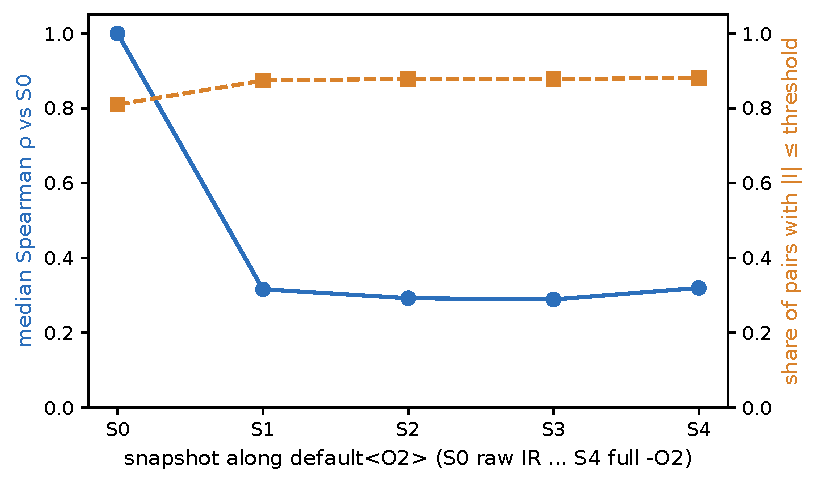
\includegraphics[width=0.49\columnwidth]{figures/v3_1_drift_decay.pdf}\hfill
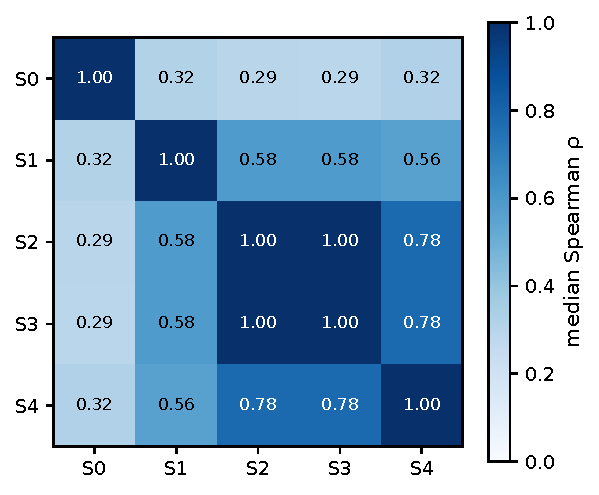
\includegraphics[width=0.47\columnwidth]{figures/v3_1_drift_matrix.pdf}
\caption{Drift along LLVM's \Otwo{} pipeline (exploratory). Left: median per-program Spearman
$\rho$ with S0 and the share of weak pairs. Right: median $\rho$ between every pair of snapshots.}
\label{fig:drift}
\end{figure}

\subsection{H3: Per-program interactions are predictable}
The LOPO model's mean absolute error is \HThreeMaeModel{}, against \HThreeMaeStatic{} for the static
graph. It removes \HThreeGap\% of the static graph's error (residual $R^2 = \HThreeRsq$) and is
better on \HThreeBetter{} of \HThreePrograms{} held-out programs (worse on \HThreeWorse).
Exploratory: for single-pass gains, the quantity re-prediction uses, the model ranks passes better
than the static graph at every snapshot (median Spearman \RankModelSZero{} vs.\ \RankStaticSZero{} at
S0, and \RankModelSTwo{} vs.\ \RankStaticSTwo{} at S2).

\subsection{H4: Re-prediction does not win at ten compilations}
The strongest other method at $\E=10$, chosen by the pre-registered rule, was the GA (\texttt{\HFourOther}). Re-prediction's IR count is \HFourRatio{} times
the GA's (\HFourWorse\% worse; better on \HFourWins{} programs, worse on \HFourLosses{}; Holm
$p=\HFourPHolm$). H4 is not supported. Figure~\ref{fig:curves} shows all methods across budgets.

\begin{figure}[t]
\centering
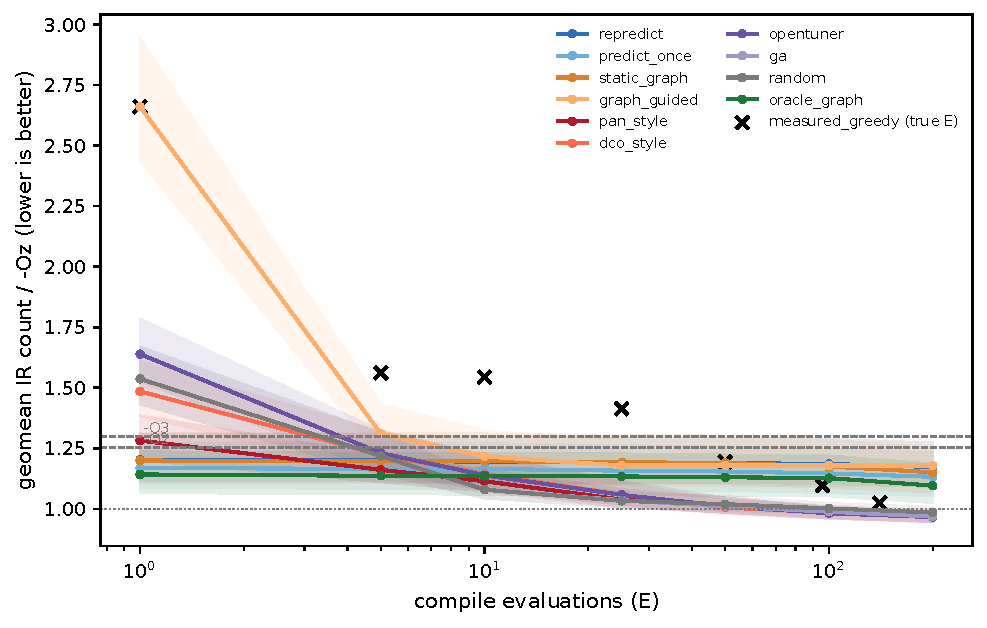
\includegraphics[width=\columnwidth]{figures/v3_1_budget_curves.pdf}
\caption{Best-so-far IR instruction count relative to \Oz{} (geomean over programs; lower is better)
by compile budget \E.}
\label{fig:curves}
\end{figure}

\subsection{Exploratory: why re-prediction loses}
The predictions are not the weak part (H3). The bottleneck is turning a graph into sequences.
\begin{itemize}
\item \textbf{Graph builders plateau.} From $\E=1$ to $\E=200$ the median per-program improvement is
\PlateauRepredict\% for re-prediction, \PlateauPredOnce\% for predict-once, \PlateauOracle\% for the
oracle graph and \PlateauStatic\% for the static graph. The GA improves by \PlateauGA\% and OpenTuner
by \PlateauOpenTuner\%. A pairwise additive estimate ranks a narrow family of similar sequences, and
spending more budget only walks down that family.
\item \textbf{Even perfect pair information does not beat search at $\E=10$.} The oracle graph's
ratio to the GA is \XOracleGARatio{} (CI \XOracleGALo--\XOracleGAHi, $p=\XOracleGAP$).
\item \textbf{Re-conditioning adds nothing under this builder.} Re-prediction vs.\ the static graph
gives \XRepStaticRatio{} ($p=\XRepStaticP$). Against predict-once it gives \XRepOnceRatio.
\item \textbf{At one compilation, predicted graphs win.} At $\E=1$ the strongest search method is
Pan-style. Predict-once beats it on \XOnceEOneWins{} of \XOnceEOnePrograms{} programs (ratio
\XOnceEOneRatio, CI \XOnceEOneLo--\XOnceEOneHi, $p=\XOnceEOneP$). Re-prediction gives
\XRepEOneRatio{} ($p=\XRepEOneP$) and the oracle graph \XOracleEOneRatio. By $\E=5$ the advantage is
gone (predict-once vs.\ Pan-style: \XOnceEFiveRatio).
\end{itemize}

\section{Discussion and Future Work}
\label{sec:discussion}

\paragraph{What a static graph misses.}
H1--H3 together say that a single interaction graph leaves a measurable, predictable share of the
signal unused. Interactions depend on the program (H1, and the variance decomposition) and on how
far optimization has progressed (H2). Both effects can be learned from other programs (H3). The
drift is concentrated in the first simplification stage. This suggests that graphs should at
least be measured on simplified IR rather than on raw front-end output.

\paragraph{Why the method did not follow.}
H4 failed. The exploratory analysis points to a specific cause: graph-to-sequence builders score a
whole sequence by summing pairwise estimates. That ranks only a narrow family of near-identical
sequences, so additional budget is wasted. Better information (re-prediction, or even the oracle
graph) cannot fix a builder that does not explore. Search methods explore well but start from
nothing: at $\E=1$ they are far behind predicted graphs.

\paragraph{Proposal: prediction-seeded search.}
These observations suggest combining the two: a search, such as a GA or OpenTuner, whose initial
population is seeded with the top sequences of the program's predicted graph, and whose mutations
are drawn from that graph. Such a search would start where predict-once is strong and keep
improving the way search does. A static-graph variant of the same search would isolate the value
of per-program prediction. We have \emph{not} evaluated this design; it is a proposal. Testing it
would need its own pre-registration and held-out programs, because the idea came from the results
reported here.

\paragraph{Size versus speed.}
Optimizing IR instruction count is a code-size objective. The GA's sequences at $\E=200$ have
\MGAOThreeSizePct\% smaller x86-64 \texttt{.text} than \Othree{}. However, they execute
\MGAOThreeDynWorse\% more instructions and run \MGAOThreeRuntimeWorse\% slower. They have
\MGAOzIRPct\% fewer IR instructions than \Oz{}, yet \MGAOzSizeWorse\% larger x86-64 \texttt{.text}.
We attribute part of that gap to backend size heuristics: \Oz{} IR carries the \texttt{minsize}
attribute, which the backend honours. Our results therefore speak to IR- and code-size-oriented
ordering, the setting of embedded targets, not to speed.

\section{Threats to Validity}
\label{sec:threats}

\paragraph{IR count as the objective.}
All four hypotheses use IR instruction count. We confirm the H1 headroom in \texttt{.text} size on
two ISAs. For executed instructions and wall-clock time, the evidence is only suggestive. Searched
sequences that minimise IR count are slower than \Othree{} (\S\ref{sec:discussion}).

\paragraph{One compiler version, one machine.}
All results come from LLVM~\LLVMVersion{} on one x86-64 laptop. AArch64 numbers are compile-only
code size. Other LLVM versions change the pass pipeline and could change the interactions.

\paragraph{Timing noise.}
Timing ran under WSL2 on a laptop: serial, pinned to one core, with 20 runs per binary in a
randomised order. Across \NRuntimeBinaries{} timed binaries the median coefficient of variation is
\RuntimeCV\%, but \RuntimeNoisy{} binaries (\RuntimeNoisyPct\%) exceed 5\%. Background load on the
host varied during the timing stage. Randomised order spreads that drift across methods, but it
adds noise~\cite{mytkowicz2009}. No hypothesis depends on timing.

\paragraph{Reimplemented baselines.}
DCO-style and Pan-style are our reimplementations of the published ideas under a common budget and
evaluator, not the original systems. We do not compare against the numbers in those papers.

\paragraph{Corpus.}
\NPrograms{} programs from four suites, \NOwn{} of them small kernels. Results may differ on
large applications. Leave-one-program-out evaluation keeps each program unseen by its own model and
graphs. Programs from the same suite can still be similar, so the static graph shares that
advantage.

\section{Related Work}
\label{sec:related}

\paragraph{Phase ordering and search.}
Almagor et al.~\cite{almagor2004} showed that program-specific sequences found by search beat a
fixed sequence, and characterised the search space. OpenTuner~\cite{opentuner} provides ensemble
search for autotuning and is a standard baseline. Ashouri et al.~\cite{ashouri2018survey} survey
machine-learning approaches to optimization selection and phase ordering.

\paragraph{Learned ordering.}
Kulkarni and Cavazos~\cite{kulkarni2012} learn a per-method ordering policy in a dynamic compiler.
MILEPOST GCC~\cite{milepost} predicts optimizations from program features. MLGO~\cite{mlgo}
replaces individual LLVM heuristics with learned policies. CompilerGym~\cite{compilergym} exposes
LLVM phase ordering as a reinforcement-learning environment. IR2Vec~\cite{ir2vec} provides the IR
embeddings we use as one feature representation.

\paragraph{Pass-interaction graphs.}
Closest to our work, DCO~\cite{dco2024} builds a dependence graph of passes from pairwise
performance dependence and searches over the resulting sub-sequences. Pan et
al.~\cite{pan2025synergy} mine a synergy knowledge graph over LLVM passes and use it to guide a
genetic algorithm. Both derive one graph from a training corpus. We measure, under a
pre-registered protocol, how much that choice costs per program and along the pipeline. We use
reimplementations in their style as baselines.

\section{Conclusion}

A single pass-interaction graph does not fit all programs. In a pre-registered study of \NPrograms{}
programs in LLVM, interactions were program-specific, with headroom that reaches code size on x86-64
and AArch64. They drifted as optimization proceeded, with the sharpest change in early simplification, and they
were predictable from other programs. Re-predicting them along the pipeline did not beat a genetic
algorithm at ten compilations. The limit we found is the graph-based sequence builder, not the
information. This points to prediction-seeded search as the next step. The artifact will be made
available.


\bibliographystyle{ACM-Reference-Format}
\bibliography{refs}

\end{document}
